\chapter{Le projet Yuukou 2}

\section{Recherches}

\subsection{Architecture du projet}
\label{section:architectureProjet}

Le premier travail a \'et\'e la r\'eflexion sur comment mettre en place une solution pouvant communiquer avec Nagios dont une description sera faite au \S~\ref{section:nagios}.
Les figures~\ref{figure:architectureProjetServiceWeb} et~\ref{figure:architectureProjetAffichage} pr\'esentent le fruit des recherches qui ont \'et\'e faites sur la mise en place du projet \YuukouII.

\begin{figure}[!ht]
	\centering
	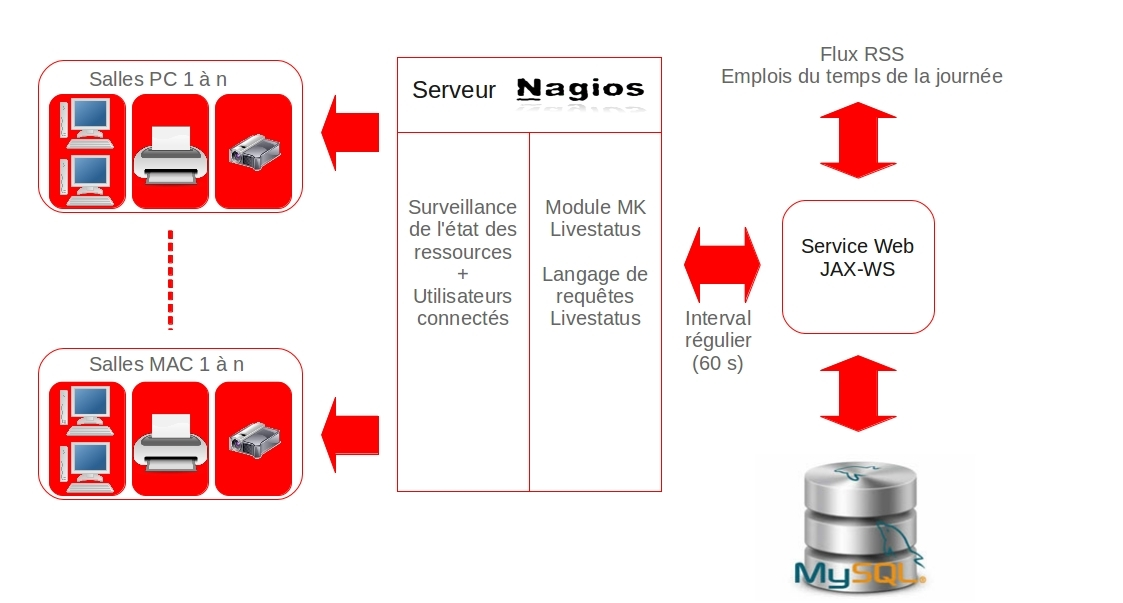
\includegraphics[scale=0.35]{architectureProjetServiceWeb.jpg}
	\caption{Architecture du projet, partie service Web}
	\label{figure:architectureProjetServiceWeb}

\end{figure}

\begin{figure}[!ht]
	\centering
	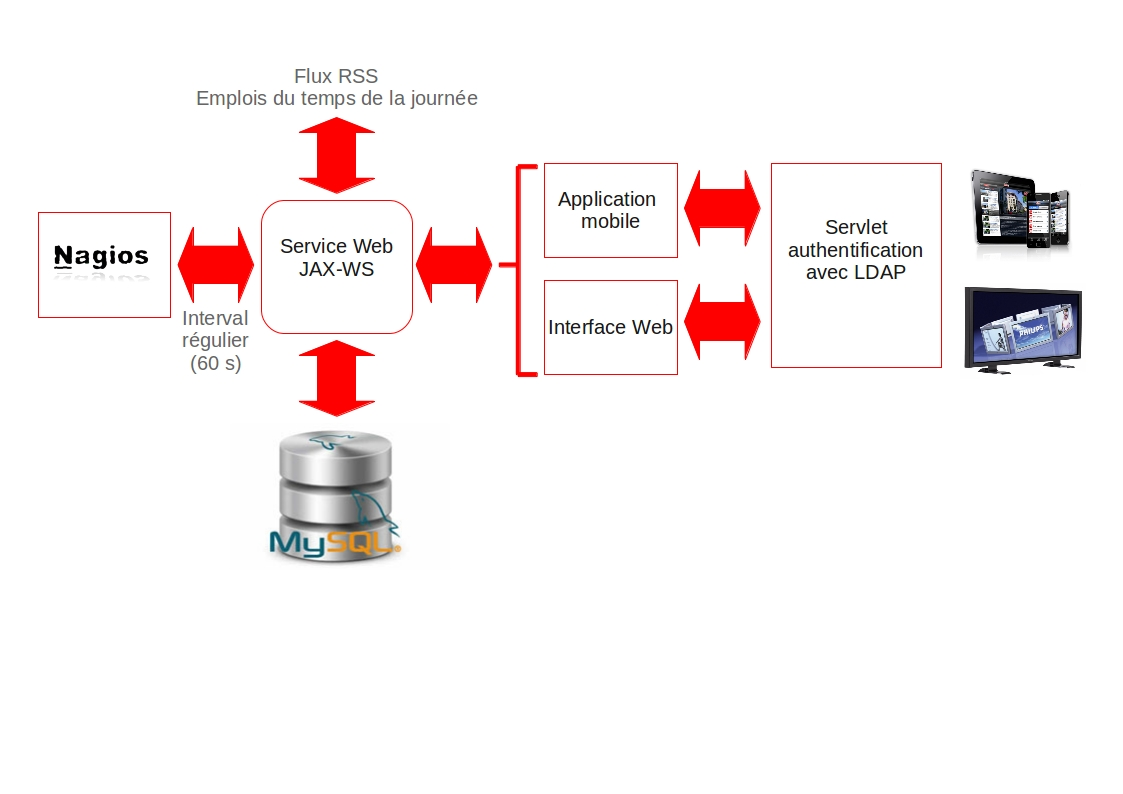
\includegraphics[scale=0.35]{architectureProjetAffichage.jpg}
	\caption{Architecture du projet, partie affichage}
	\label{figure:architectureProjetAffichage}

\end{figure}

\subsubsection{Partie service Web}

Basiquement Nagios sert \`a surveiller les ressources auxquelles il lui est permis d'acc\'eder.
De ce fait, il doit garder des traces des informations qu'il r\'ecup\`ere.
Ces informations sont stock\'ees dans un fichier.
C'est pourquoi un module existe sp\'ecialement pour acc\'eder aux informations contenu dans ce fichier. 
Le module \textit{MK Livestatus} permet \`a l'aide d'un langage de requ\^etes qui lui est propre, de r\'ecup\'erer les informations que garde Nagios.

Le service Web doit permettre, dans un premier temps, de r\'ecup\'erer toutes les informations utiles pour un archivage des donn\'ees.
Elles sont stock\'ees dans une base de donn\'ees MySQL.
\noindent Ces informations sont :

\begin{itemize}
	\item les donn\'ees r\'ecup\'er\'ees via le module \textit{MK Livestatus}, la r\'ecup\'eration doit \^etre faite \`a intervalles r\'eguliers;
	\item les diff\'erents emplois du temps de toutes les salles que Nagios surveille, la r\'ecup\'eration doit \^etre faite une fois par jour;
	\item les donn\'ees sur un utilisateur inconnu (nom, pr\'enom, r\^ole : \'etudiant par exemple, photo) via un serveur LDAP.

\end{itemize}

\subsubsection{Partie affichage}

Dans un deuxi\`eme temps, le service Web doit pouvoir retourner ces informations tri\'ees \`a un utilisateur normal ou un administrateur afin de garantir l'affichage sous la forme d'une application mobile ou d'une interface Web.
La r\'eflexion doit ainsi se porter sur le contenu des diff\'erentes m\'ethodes auxquelles un utilisateur pourra avoir acc\`es (en fonction qu'il soit administrateur ou non).
Le but \'etant un affichage le plus rapide possible des informations demand\'ees.

L'utilisateur doit s'authentifier via un Servlet$^*$ qui communique avec LDAP$^*$ et qui donne un acc\`es \`a l'application.
Le reste de la communication est s\'ecuris\'ee comme expliqu\'e dans le \S~\ref{section:securisation}.

Le dernier point est de choisir un format pour les donn\'ees qui seront \'echang\'ees entre le service Web et l'application cliente.

C'est sur cette partie que Yacine MAGHEZZI est intervenu durant son stage.

\subsection{Nagios}
\label{section:nagios}

\begin{figure}[!ht]
	\centering
	
\includegraphics[scale=0.5]{nagiosLogo.jpg}
	\caption{Logo de Nagios}

\end{figure}

\subsubsection{Pr\'esentation}

Nagios est une application permettant la surveillance syst\`eme et r\'eseau de toute une infrastructure informatique.
Nagios compl\`ete cette surveillance en offrant la possibilit\'e d'alerter les \'equipe en charge de l'infrastructure en cas d'apparition de probl\`emes comme une panne ou encore un fonctionnement anormal.
C'est actuellement la solution de surveillance la plus efficace du march\'e.

\parpic{
	\begin{minipage}{0.20\textwidth}
		
\includegraphics[scale=0.6]{netsaintLogo.jpg}
	\end{minipage}}
Nagios a \'et\'e cr\'e\'e en 1999 et portait initialement le nom de \textit{NetSaint Network Monitor}.
Il est \'ecrit en C et est con\c{c}u pour un environnement Unix.
Le projet a \'et\'e maintenu jusqu'en 2002 avant de changer de nom pour devenir Nagios en r\'eponse \`a une contestation judiciaire par les propri\'etaires d'une marque similaire.
N.A.G.I.O.S. est l'acronyme r\'ecursif de \og{}\textit{Nagios Ain't Gonna Insist On Sainthood}\fg{} o\`u Sainthood est une r\'ef\'erence \`a \textit{NetSaint}.

Maintenant connu sous le nom de Nagios XI, Nagios est un logiciel libre sous la licence GNU GPL V2. 
Il est actuellement disponible sur son site Internet\cite{biblio:siteNagios} en version 3.2.1.

\subsubsection{Fonctionnement}

\noindent L'architecture de base de Nagios est tr\'es simple, elle comporte :

\begin{itemize}
	\item un ordonnanceur pour g\'erer les v\'erification ainsi que les actions \`a prendre sur les diff\'erents incidents;
	\item une partie graphique : visible \`a travers un simple serveur Web;
	\item des sondes : greffons (ou \textit{plugins} en anglais) dans Nagios, ce sont de petits \textit{scripts} permettant d'effectuer diverses v\'erifications.

\end{itemize}

\vspace{0.20cm}

\`A la base, Nagios est un moteur d'ordonnancement de v\'erifications diverses et vari\'ees dont les v\'erifications sont effectu\'ees via des greffons.
Ces v\'erifications peuvent \^etre la charge d'utilisation du CPU\protect\footnote{\textit{Central Processing Unit} ou processeur en fran\c{c}ais}, l'espace disque utilis\'e ou encore qui est connect\'e actuellement.
Dans le cadre de la v\'erification de l'infrastructure, deux types de machines sont observ\'ees : les ordinateurs dot\'es de Windows et les ordinateurs dot\'es de Macintosh.

Nagios \'etant install\'e et fonctionnel depuis un peu plus d'un an sur le site de New Cavendish, les greffons pour observer les deux types de machines ont d\'ej\`a \'et\'e d\'evelopp\'es.
Pour les machines fonctionnant sous Windows, le greffon est en fait l'appel \`a la commande Unix \textit{Winexe} qui permet l'ex\'ecution de commandes \`a distance sur des machines Windows.
Pour les machines fonctionnant sous Macintosh, le greffon effectue une connexion SSH\protect\footnote{\textit{SecureShell}}, offrant une connexion s\'ecuris\'ee sur une machine distante pour ensuite ex\'ecuter la commande Unix \textit{who} permettant l'obtention de l'utilisateur connect\'e.

\subsubsection{\og{}Monitoring\fg{} \`a l'universit\'e}

Initialement, Nagios surveillait juste les machines se situant sur le campus de New Cavendish, soit 31 salles PC seulement machines.
Actuellement, ce sont 102 salles qui sont sous la surveillance de Nagios, soit 99 salles utilisant Windows soit 1920 PC, 3 salles utilisant des Macintosh soit 63 MAC, pour un total de 1983 machines \`a travers toute l'universit\'e : la grande majorit\'e des ordinateurs de l'universit\'e.
Il faut noter que seuls les Macintosh de New Cavendish sont sous surveillance, les autres n\'ecessitant d'\^etre list\'es et des acc\`es diff\'erents.
De ce fait, le nombre de machines devrait augmenter par la suite.

\subsubsection{Vue sur la surveillance de Nagios}




TODO REPRENDRE



\section{La notion de service Web}
\label{section:serviceWeb}

\subsection{D\'efinition}

Un service Web est une application accessible par le r\'eseau, qui permet \`a un client de dialoguer avec le service Web et cela ind\'ependamment de tout langage de programmation et de toute plate-forme d'ex\'ecution.
Un service Web d\'evelopp\'e en Java peut donc \^etre accessible par un client PHP$^*$ par exemple.
C'est un syst\`eme de messagerie standard utilisant le protocole HTTP pour communiquer \`a travers le r\'eseau et s'\`echangeant des fichiers XML.
Son int\'er\^et resulte dans l'utilisation de normes (HTTP et XML) permettant l'int\'erop\'erabilit\'e des services.
De plus, le fait que les services Web n'imposent pas de mod\`ele de programmation sp\'ecifique permet aux vendeurs d'outils de d\'eveloppement d'offrir des m\'ethodes diff\'erentes et donc de facilement diff\'erencier leurs produits de ceux de leurs concurrents.

\subsection{Architecture}

Lorsqu'on parle de services Web, on parle aussi de SOA, \textit{Service-Oriented Architecture} ou architecture orient\'ee services en fran\c{c}ais.
Une architecture orient\'ee services est un style d'architecture qui a pour objectif une interd\'ependance faible entre diff\'erents agents logiciels (module, services).
Les services Web poss\`edent trois normes principales qui sont SOAP, WSDL et UDDI qui permettent respectivement la fa\c{c}on dont les messages sont \'echang\'es, sa description et sa d\'ecouverte.

\subsubsection{\'Echange de messages}

Dans la grande majorit\'e des services Web, le protocole principal de communication est SOAP\protect\footnote{\textit{Simple Object Access Protocol}}.
Il offre le transport d'objets s\'erialis\'es (objets repr\'esent\'es par un flux de bytes) et autres donn\'ees en XML, et l'appel de proc\'edures distantes.

\subsubsection{Description d'un service Web}

Un service Web est d\'ecrit par un document WSDL\protect\footnote{\textit{Web Services Description Language}}.
C'est un langage de description bas\'e sur XML qui permet de donner de fa\c{c}on pr\'ecise les d\'etails concernant le service Web :

\begin{itemize}
	\item son protocole de communication utilis\'e;
	\item le format de messages requis pour communiquer avec le service Web;
	\item les m\'ethodes que le client peut utiliser;
	\item sa localisation.

\end{itemize}

\vspace{0.20cm}

\noindent Un fichier WSDL permet ainsi de savoir comment communiquer avec le service Web.

\subsubsection{D\'ecouverte d'un service Web}

Pour utiliser un service Web, il faut savoir s'il existe.
UDDI\protect\footnote{\textit{Universal Description, Discovery and Integration Service}} est une norme qui d\'efinit le m\'ecanisme pour d\'ecouvrir dynamiquement des services Web.
C'est en fait un annuaire de services permettant de localiser sur le r\'eseau le service Web demand\'e.
\noindent Il comporte :

\begin{itemize}
	\item \textit{des pages blanches}, liste des entreprises ainsi que les informations les concernant;
	\item \textit{des pages jaunes}, liste des services Web de chacunes des entreprises sous le format WSDL
	\item \textit{des pages vertes}, liste des informations techniques pr\'ecises sur les services fournis.

\end{itemize}


\subsection{Fonctionnement}

Le fonctionnement des services Web s'articule autour de trois acteurs principaux illustr\'es par la figure~\ref{figure:schemaServiceWeb}.

\begin{figure}[!ht]
	\centering
	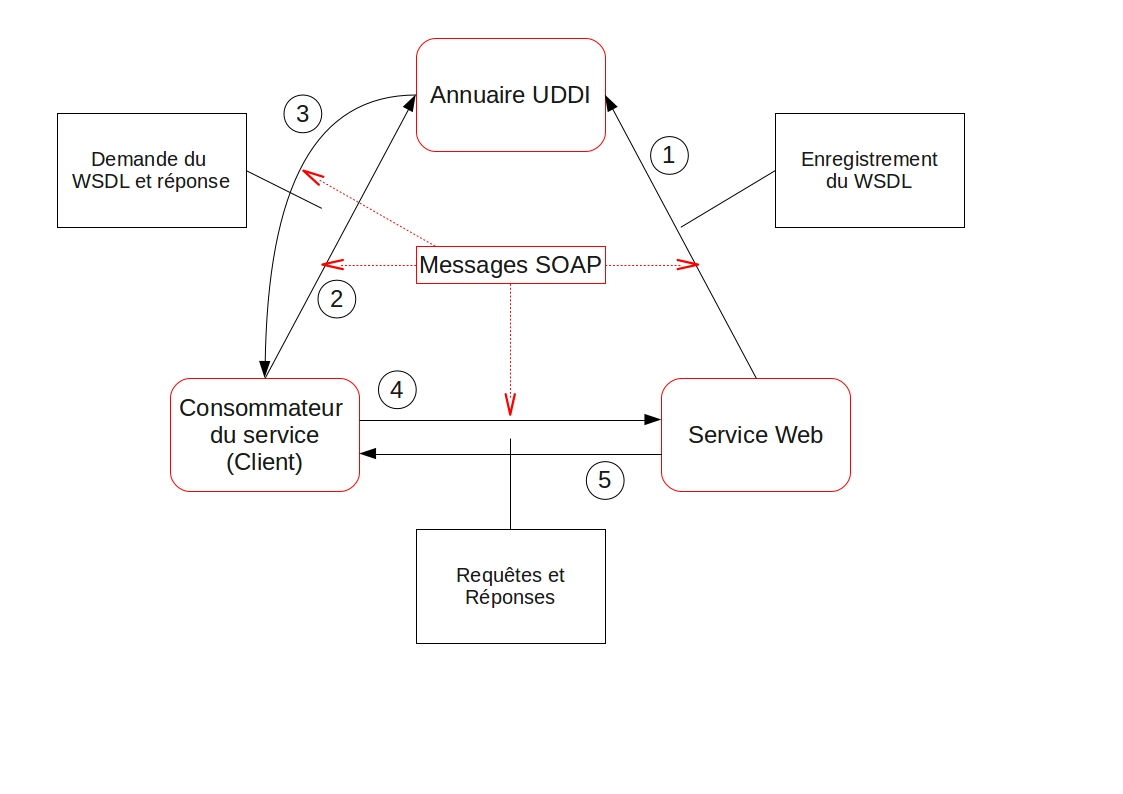
\includegraphics[scale=0.35]{schemaServiceWeb.jpg}
	\caption{Fonctionnement des services Web}
	\label{figure:schemaServiceWeb}

\end{figure}

Les \'etapes impliquant la mise \`a disposition et l'utilisation (consommation) d'un service Web sont les suivantes :

\begin{enumerate}
	\item le service Web d\'ecrit son service en utilisant WSDL. 
	Cette d\'efinition est publi\'ee dans l'annuaire UDDI;
	\item le client envoit une ou plusieurs requ\^ete afin de localiser le service Web \`a l'annuaire et d\'eterminer comment communiquer avec ce service;
	\item une partie du fichier WSDL fourni par le service Web est pass\'e au client. 
	Le client peut maintenant savoir quelles requ\^etes et r\'eponses envoyer au service Web;
	\item le client utilise le fichier WSDL pour envoyer une requ\^ete au service Web;
	\item le service Web fournit la r\'eponse attendue au client.

\end{enumerate}

\subsection{L'API JAX-WS}

Java API$^*$ for XML Web Services (JAX-WS) est une API Java permettant de simplifier la cr\'eation, le d\'eveloppement et le d\'eploiement de services Web clients et de services Web prestataires.
Il fonctionne avec un syst\`eme d'annotations sp\'ecifique du code Java.
JAX-WS fait partie de la plate-forme Java EE\protect\footnote{\textit{Java Platform, Entreprise Edition}} de Sun Microsystems.
Anciennement appel\'ee JAX-RPC\protect\footnote{\textit{Java API for XML-based RPC}}, ce changement de nom intervient lors de l'abandon du style RPC\protect\footnote{\textit{Remote Procedure Call}}, des appels de proc\'edures distantes, pour des services Web de style document, avec une transmission de donn\'ees au format XML d\'efinies dans un sch\'ema XML.

Toute la partie communication de JAX-WS est g\'er\'ee avec des messages de type SOAP \`a travers HTTP.
L'API$^*$ permet de cacher toute la complexit\'e des messages, le d\'eveloppeur choisit simplement la mani\`ere d'impl\'ementer le service. 
Pour cela, il existe deux m\'ethodes : top-down et bottom-up.

La m\'ethode top-down permet de d\'evelopper un service Web en partant d'un fichier WSDL.
Ce fichier doit contenir la compl\`ete description de tout le service Web, ensuite le code Java est g\'en\'er\'e automatiquement.
Les classes doivent ensuite \^etre compl\'et\'ees avant d\'eploiement.

La m\'ethode bottom-up permet quant \`a elle de d\'evelopper un service Web en partant du code Java.
Le code Java est d'une part annot\'e, ensuite le fichier WSDL est automatiquement g\'en\'er\'e.
Le service peut enfin \^etre d\'eploy\'e.

C'est la m\'ethode bottom-up qui a \'et\'e employ\'ee dans le projet.
Elle permet de ne se soucier que du code Java, le reste \'etant g\'er\'e automatiquement par NetBeans avec la construction du service Web et le d\'eploiement sur le serveur GlassFish.
Le code~\ref{code:exempleJAXWS} donne un exemple d'annotations sur un code Java.

\vspace{0.20cm}

\lstinputlisting[language=Java]{codes/ExempleService.java}
\captionof{figure}{Exemple de classe Java annot\'ee avec JAX-WS}
\label{code:exempleJAXWS}

JAX-WS \textit{Reference Implementation} est actuellement disponible sur son site Internet\cite{biblio:siteJAXWS} en version 2.2.6.

\subsection{L'IDE NetBeans}

\begin{figure}[!ht]
	\centering
	
\includegraphics[scale=0.25]{netbeansLogo.jpg}
	\caption{Logo de NetBeans}

\end{figure}

NetBeans est un IDE\protect\footnote{\textit{Integrated Development Environment}}$^*$ open source d\'evelopp\'e par Sun Microsystems permettant le d\'eveloppement en utilisant les langages de programmation tels que Java, JavaScript, PHP$^*$, C, C++, et autres.
Il est \'ecrit en Java et fonctionne sous Windows, Mac OS, Linux, Solaris et d'autres plates-formes du moment qu'elles poss\`edent une JVM\protect\footnote{\textit{Java Virtual Machine}}$^*$ compatible.

NetBeans permet de d\'evelopper et d\'eployer rapidement des applications graphiques Swing, des Applets, des JSP/Servlets et des architectures J2EE\protect\footnote{\textit{Java Platform, Enterprise Edition}}.
Il poss\`ede toutes les fonctionnalit\'es recherch\'ees dans un IDE$^*$ moderne (coloration syntaxique, refactoring, d\'ebogueur, \ldots) et ajoute, dans le cas d'un d\'eveloppement d'un service Web comme pour ce projet, un support avec la derni\'ere version de GlassFish, permettant notamment de faire des \og{}deploy on save\fg{}, de d\'eployer les applications Web sur un serveur distant et de contr\^oler le serveur (suivre la sortie de logs, d\'emarrer, arr\^eter le serveur). 
Il donne acc\`es \`a une gestion simple du serveur d'application GlassFish qui sera utilis\'e dans le projet.
Sa premi\`ere version date de 1996 et portait le nom Xelfi. 
Il est actuellement disponible sur son site Internet\cite{biblio:siteNetbeans} en version 7.1.2.

\subsection{Le serveur Web GlassFish}

\begin{figure}[!ht]
	\centering
	
\includegraphics[scale=0.35]{glassfishLogo.jpg}
	\caption{Logo de GlassFish}

\end{figure}

GlassFish est un serveur d'application open source d\'evelopp\'e par Sun Microsystems pour les plates-formes Java EE\protect\footnote{\textit{Java Platform, Entreprise Edition}} 5 et 6, et est maintenant maintenu par Oracle Corporation.
Il dispose de nombreux outils pour faciliter le d\'eveloppement, le d\'eploiement et la maintenance d'application.
Un de ses avantages est qu'il est particuli\`erement bien int\'egr\'e \`a NetBeans, ce qui permet un d\'eploiement tr\`es rapide des applications ainsi qu'une trace d'ex\'ecution lors du fonctionnement.
GlassFish est disponible sur son site Internet\cite{biblio:siteGlassfish} en version 3.1.2.

\subsection{Le SGBD MySQL}

\subsection{L'acc\`es aux donn\'ees des tables}

Par souci de performance, \cad, limiter les acc\`es multiples \`a la base de donn\'ees mais aussi faciliter la manipulation des donn\'ees lors des traitements, le design pattern$^*$ \textit{Data Access Object} (DAO) a \'et\'e utilis\'e.
Un Data Access Object, ou objet d'acc\`es aux donn\'ees en fran\c{c}ais, est un objet qui constitue une repr\'esentation en m\'emoire des donn\'ees d'une base de donn\'ees.
En Java, un DAO est une classe repr\'esentant une table dont les attributs sont les champs de la table comme le montre la figure~\ref{figure:dao}.
Des classes repr\'esentant des listes sont g\'en\'eralement d\'evelopp\'e pour contenir les DAO et simplifier l'acc\`es aux donn\'ees.

Lorsqu'il sera n\'ecessaire d'effectuer des traitements r\'ep\'et\'es sur les donn\'ees d'une table, m\^eme si ces traitements ne portent pas sur la totali\'e de la table, il est pr\'ef\'erable de charger en m\'emoire la totalit\'e des \'el\'ements utiles avec, dans le cas id\'eal, une seule requ\^ete SQL$^*$.

\begin{figure}[!ht]
	\centering
	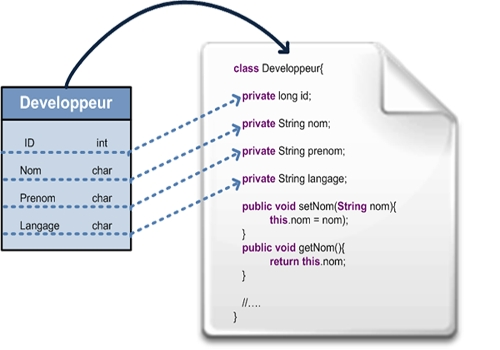
\includegraphics[scale=0.5]{dao.jpg}
	\caption{Exemple de \textit{mapping} d'une table avec sa classe DAO associ\'ee (\textit{source : Cyrille Herby})}
	\label{figure:dao}

\end{figure}

Dans le cadre du projet, les chargements sont effectu\'es lorsqu'un client appelle une m\'ethode du service Web. 
Les donn\'ees sont charg\'ees dans une liste, elles sont ensuite trait\'ees puis retourn\'ees au client.

\subsection{Le format de retour}
\label{section:formatRetour}

Le choix du type de retour est un choix important.
En effet, il faut que les donn\'ees puissent \^etre rapidement transmises, r\'ecup\'er\'ees, trait\'ees et affich\'ees.
L'objectif est un affichage instantan\'e des pages sur le navigateur Web ou l'application mobile.
De ce fait, plusieurs possibilit\'es ont \'et\'e envisag\'ees.


\subsubsection{{\og}\textit{Parsing}{\fg} d'un texte}

La premi\`ere est de transmettre un document texte basique, celui-ci format\'e d'une certaine fa\c{c}on afin d'\^etre \textit{pars\'e} ({\cad} parcourir un flux structur\'e d'informations pour en extraire les donn\'ees).
Ce qui aurait comme avantage de pouvoir \^etre r\'ecup\'er\'e par un client utilisant n'importe quel langage.
La figure~\ref{code:exemplePlaintext} repr\'esente une exemple de fichier qu'il est facile de \textit{parser}, il suffit de r\'ecup\'erer les informations se trouvant entre les arobases.

\vspace{0.20cm}

\begin{lstlisting}[language=plaintext]
info1 @ info2 @ info3 @ info4
\end{lstlisting}
\captionof{figure}{Exemple de ligne pouvant \^etre facilement \textit{pars\'ee}}
\label{code:exemplePlaintext}

Pour r\'ecup\'erer les informations de cet exemple, il suffit de parcourir le fichier en stockant les informations contenues entre les \textbf{@}.

Cependant cette m\'ethode est assez contraignante et oblige \`a parcourir l'ensemble du fichier alors qu'un seul type d'information peut \^etre utile.
Ce qui signifie une perte de temps plus ou moins significative en fonction de la taille du fichier re\c{c}u.

\subsubsection{Objet Java s\'erialisable}

Une autre m\'ethode pourrait \^etre de transmettre un objet Java dit s\'erialisable.
La s\'erialisation est un m\'ecanisme fourni par Java permettant de consid\'erer un objet comme une s\'equence de d'octets qui inclut les donn\'ees de l'objet, le type de l'objet et le type des donn\'ees.
De cette mani\`ere, l'objet en question peut \^etre transmis \`a travers le r\'eseau vers une autre application Java pour le r\'ecup\'erer et le d\'es\'erialiser, ce qui repr\'esente la proc\'edure inverse de la s\'erialisation.
La figure~\ref{code:exempleJava} donne un exemple de classe Java s\'erialisable qui pourrait \^etre transmise par le r\'eseau comme un flux de bytes.

\vspace{0.20cm}

\lstinputlisting[language=Java]{codes/Exemple.java}
\captionof{figure}{Exemple de classe Java s\'erialisable}
\label{code:exempleJava}

L'objet contiendrait toutes les donn\'ees utiles et celles-ci seraient facilement accessibles.
Le probl\`eme venant avec cette solution est que les objets doivent \^etre r\'ecup\'er\'es par une JVM$^*$.
Ce qui peut s'av\'erer plus ou moins compliqu\'e voir impossible dans d'autres langages de programmation que Java.

\subsubsection{XML}

eXtensible Markup Language ou XML est un m\'eta langage pour r\'ealiser du balisage g\'en\'erique permettant de mettre en forme les documents. XML a connu un grand succ\`es depuis sa cr\'eation.
Il est utilis\'e en particulier pour g\'erer la configuration, le stockage des donn\'ees, l'\'echange d'informations et bien d'autres fonctions encore.
La figure~\ref{code:exempleXML} donne un exemple de document XML pouvant \^etre facilement converti en une arborescence DOM$^*$.

\vspace{0.20cm}

\lstinputlisting[language=XML]{codes/Exemple.xml}
\captionof{figure}{Exemple de document XML}
\label{code:exempleXML}

XML offre une solution structur\'ee et tr\`es simple \`a comprendre pour l'envoi d'information par le r\'eseau, cependant dans les \'echanges d'informations entre client et serveur, il montre ses limites :

\begin{itemize}
	\item le chargement et la manipulation deviennent vite compliqu\'es, la plupart du temps il est n\'ecessaire de \textit{parser} le XML sous forme de DOM$^*$, puis de le parcourir, ce qui requiert l'appel de nombreuses fonctions, sans mentionner le fait que \textit{parser} un document XML est parfois long;
	\item la taille des fichiers \'echang\'es peut parfois \^etre cons\'equente du fait de la duplication des donn\'ees : par nature, le XML ne permet pas de g\'erer une \'enorme masse d'informations.

\end{itemize}

\subsubsection{JSON}

JavaScript Object Notation ou JSON est un format l\'eger d'\'echange de donn\'ees texte.
Il utilise la notation des objets JavaScript pour transmettre de l'information structur\'ee.
Il est aussi souvent utili\'e pour simplifier et all\'eger les acc\`es \`a des services Web depuis les navigateurs.
La figure~\ref{code:exempleJSON} donne une exemple de fichier JSON reprenant le m\^eme arbre que le document XML de la figure~\ref{code:exempleXML}.

\vspace{0.20cm}

\lstinputlisting[language=JSON]{codes/Exemple.json}
\captionof{figure}{Exemple de fichier JSON}
\label{code:exempleJSON}

\subsubsection{Choix du format}

Le choix du format de retour des donn\'ees s'est port\'e sur l'utilisation de JSON.
Le but du client, qui demande des informations au service Web, est de recevoir les donn\'ees le plus rapidement possible afin d'avoir \`a les afficher dans la foul\'ee.
De ce fait, le \textit{parsing} d'un texte contenant des balises \`a certains endroits s'av\`ere inadapt\'e, notamment pour r\'ecup\'erer un seul type d'information.
L'envoi d'un objet s\'erialisable Java est, quant \`a lui trop restrictif. Le choix a donc \'et\'e de choisir entre XML ou JSON.

XML offre un format de donn\'ees verbeux et prend beaucoup d'espace. 
De plus un document XML peut \^etre valid\'e via l'utilisation de DTD\protect\footnote{\textit{Document Type Definition}}, document permettant de d\'ecrire un mod\`ele de document XML, ou de XSD\protect\footnote{\textit{XML Schema Definition}}, langage de description de format de document XML permettant de d\'efinir la structure et le type de contenu d'un document XML.

JSON offre un format de fichier plus simple que XML, facilement compr\'ehensible.
Pour compl\'eter, les fichiers JSON, \`a arbre \'egal, seront toujours plus petits que l'\'equivalent XML et pr\'esenteront l'avantage d'\^etre plus rapidement \textit{pars\'es}.

Au final JSON permet une plus grande rapidit\'e dans les \'echanges avec un serveur ainsi que sur le temps de \textit{parsing} des fichiers, le tout avec une \'economie des ressources du fait de sa petit taille.
Cependant, les donn\'ees ne peuvent pas \^etre v\'erifi\'ees dans un fichier JSON, il demande donc une certaine rigueur dans son \'ecriture du cot\'e serveur ainsi qu'une connaissance de sa structure du cot\'e client.

\subsection{Compl\'ement d'information sur JSON}

\subsubsection{Pr\'esentation}

Une courte description de ce qu'est JSON a d\'ej\`a \'et\'e faite au \S~\ref{section:formatRetour}.
Pour reprendre ce qui a d\'ej\`a \'et\'e dit, JSON est un format l\'eger d'\'echange de donn\'ees qui est apparu en 2002.
Il est facile \`a \'ecrire et comprendre pour des humains.
Il est bas\'e sur un sous-ensemble du langage de programmation JavaScript et est compl\`etement ind\'ependant de tout langage, tout en poss\`edant des conventions famili\`eres aux langages descendant du C (C++, C\#, Java, JavaScript, \ldots).
Ces propri\'et\'es font de JSON un langage d'\'echange de donn\'ees id\'eal.

Cependant, il ne supporte pas les espaces de noms au contraire d'XML.
Pour la v\'erification des donn\'ees, les sch\'emas JSON ne sont pas tr\`es utilis\'es du fait qu'ils doivent \^etre ecrit \`a la main comme il n'existe aucun outil pour g\'en\'erer un sch\'ema \`a partir de donn\'ees JSON.
Et concernant la s\'ecurit\'e, il existe la possibilit\'e o\`u des \textit{scripts} malveillants pourraient \^etre dissimul\'es et ex\'ecut\'es.
Il existe des fonctions pour tester les fichiers JSON mais celles-ci ne sont pas vraiment concluantes.
La meilleure d\'efense est de conna\^itre \`a l'avance les points sensibles et de prendre les pr\'ecautions n\'ecessaires.

\subsubsection{Structure}

JSON se base sur deux structures de donn\'ees universelles dans pratiquement tous les langages de programmation modernes :

\begin{itemize}
	\item une collection de couples nom/valeur;
	\item une liste de valeurs ordonn\'ees.

\end{itemize}

\vspace{0.20cm}

\noindent Ces \'el\'ements repr\'esentent trois types de donn\'ees :

\begin{itemize}
	\item un \textit{objet} :\\Ensemble de couples nom/valeur non ordonn\'es. Un objet commence par \textsf{\{ (accolade gauche)} et se termine par \textsf{\} (accolade droite)}.
	Chaque nom est suivi de \textsf{: (deux-points)} et les couples nom/valeur sont s\'epar\'es par \textsf{, (virgule)};
	\item un \textit{tableau} :\\Collection de valeurs ordonn\'ees. Un tableau commence par \textsf{$[$ (crochet gauche)} et se termine par \textsf{$]$ (crochet droit)}.
	Les valeurs sont s\'epar\'ees par \textsf{, (virgule)};
	\item une \textit{valeur} :\\Soit une \textsf{cha\^ine de caract\`eres} entre guillemets, soit un \textsf{nombre}, soit \textsf{true} ou \textsf{false} ou \textsf{null}, soit un \textsf{objet}, soit un \textsf{tableau}.
	Ces structures peuvent \^etre imbriqu\'ees;
	\item une \textit{cha\^ine de caract\`eres} :\\Suite caract\'eres Unicode (z\'ero ou plus), entre guillemets, et utilisant les \'echappements avec antislash. 
	Un caract\`eres est repr\'esent\'e par une cha\^ine d'un seul caract\`ere.

\end{itemize}

\section{Communication avec Nagios}

Nagios offre la surveillance d'un grand ensemble de machines dans l'universit\'e. 
Cependant s'il n'y a aucune mani\`ere de r\'ecup\'erer ces informations, il n'aurait aucune utilit\'e dans le projet.
Ainsi un module a \'et\'e d\'evelopp\'e, son but \'etant de pouvoir interroger Nagios et obtenir ses r\'eponses le plus rapidement et simplement possible.

\subsection{Le module MKLivestatus}
\label{section:moduleMKLivestatus}

Le module MKLivestatus permet un acc\`es imm\'ediat au statut de Nagios ainsi qu'\`a ses donn\'ees de logs.
Avant le module, une fa\c{c}on classique de r\'ecup\'erer les informations importantes \'etait de \textit{parser} le fichier \textsf{status.dat}, qui est cr\'e\'e automatique par Nagios \`a chacun de ses cycles.
Ce fichier contient toutes les informations concernant les services et les machines que Nagios surveille.
\textit{Parser} ce fichier s'av\`ere d\'elicat, surtout pour extaire quelques informations.
Il existe bien une mani\`ere alternative de r\'ecup\'erer ces informations avec le module NDO.
Ce module est directement charg\'e dans le processus de Nagios et \`a chaque nouveau cycle, il envoie les mises \`a jour via une socket UNIX$^*$ \`a un processus auxiliaire qui se charge de mettre \`a jour une base de donn\'ees.

Les avantages \'etant une mise \`a jour imm\'ediate de l'information et une simplicit\'e et rapidit\'e d'acc\`es aux bases de donn\'ees pour les applications.
Mais d'un autre cot\'e, la mise en place de ce syst\^eme est complexe, elle n\'ecessite une administration humaine de la base de donn\'ees, la consommation CPU est significative juste pour garder la base \`a jour et son entretien r\'egulier peut bloquer Nagios pendant un moment (cela d\'epend de la taille de l'infrastructure).

Le module MKLivestatus reprend le principe de NDO dans l'int\'egration directe dans le processus Nagios, cependant, la diff\'erence de taille est qu'il ouvre juste une socket de communication par laquelle les donn\'ees peuvent \^etre retrouv\'ee \`a la demande.
La socket ouverte par d\'efaut par MKLivestatus est une socket UNIX$^*$, mais il est possible de configurer une socket Internet classique sur un port choisi et accessible seulement par certaines machines.
Par cette socket, il est possible d'envoyer une requ\^ete vers une cible sp\'ecifique comme un service, une machine, un ensemble de machines, \ldots{}
La r\'eponse est imm\'ediate et les donn\'ees renvoy\'ees ont \'et\'e directement lu dans les structures de donn\'ees internes de Nagios.

\noindent MKLivestatus offre donc de nombreux avantages :

\begin{itemize}
	\item consommation CPU non mesurable, juste une petite consommation lors de l'ex\'ecution d'une requ\^ete;
	\item pas d'ecritures sur le disque;
	\item acc\`es aux donn\'ees beaucoup plus rapide qu'avec un \textit{parsing} du fichier \textsf{status.dat} ou l'ex\'ecution de requ\^etes SQL$^*$.
	\item pas de configuration, d'administration ou autre, tout est install\'e automatiquement.

\end{itemize}

\vspace{0.20cm}

MKLivestatus est disponible sur le site Internet\cite{biblio:siteMklivestatus} de Mathias Kettner en version stable 1.1.12p7.

\subsection{Requ\^etes pour Nagios}

\subsubsection{\'Ecriture des requ\^etes avec LQL}

LQL, Livestatus Query Language, prononc\'e \og Liquel\fg, est un langage sp\'ecialement con\c{c}u pour communiquer avec le module MKLivestatus via une socket.
Il ressemble un peu au langage SQL$^*$.

\noindent Chaque requ\^ete consiste en :

\begin{itemize}
	\item une commande commen\c{c}ant par le mot cl\'e \textsf{GET} suivit du nom de la \textit{table};
	\item un nombre arbitraire de lignes d'en-t\^ete consistant en un mot cl\'e, un double-point et une liste d'arguments;
	\item une ligne vide ou une fin de transmission (pour fermer la proc\'edure d'envoi sur la socket).

\end{itemize}

\vspace{0.20cm}

Tous les mots cl\'es sont sensibles \`a la casse. 
La version actuelle de Livestatus donne acc\`es \`a seize tables dont voici les principales :

\begin{itemize}
	\item \textbf{hosts} : les h\^otes surveill\'es par Nagios;
	\item \textbf{services} : les services de Nagios, reli\'es avec toutes les donn\'ees de la table \textit{hosts};
	\item \textbf{hostgroups} : les groupes d'h\^otes cr\'e\'es dans Nagios;
	\item \textbf{servicegroups} : les groupes de services cr\'e\'es dans Nagios.

\end{itemize}

\vspace{0.20cm}

Les requ\^etes peuvent aussi \^etre affin\'ees avec la s\'election de certaines colonnes, la cr\'eation de filtres sur les r\'esultats (tous les r\'esultats dont la valeur est \'egale \`a deux), compter des r\'esultats, faire des comparaisons avec des expressions r\'eguli\`eres, \ldots{}
Au final, LQL s'av\`ere tr\`es flexible d'utilisation.
La figure~\ref{code:exempleLQL} donne un exemple de requ\^ete permettant de r\'ecup\'erer tous les services avec leur \'etat actuel \`a 2.

\vspace{0.20cm}

\lstinputlisting[language=LQL]{codes/nagiosExemple.ngs}
\captionof{figure}{Exemple de requ\^ete LQL}
\label{code:exempleLQL}

Les \textit{scripts} Nagios utilis\'es tout au long du stage sont disponibles en annexe~\ref{chapterAnnexe:fichiersLQLNagios} de ce rapport.

\subsubsection{Ex\'ecution des requ\^etes}

Comme pour une base de donn\'ees SQL$^*$, toutes les tables poss\`edent un nombre de colonnes.
Si une requ\^ete est pass\'ee sans param\^etres, toutes les colonnes seront retourn\'ees dans l'ordre alphab\'etique.

Comme vu dans au \S~\ref{section:moduleMKLivestatus}, il existe deux mani\`eres d'acc\'eder \`a la socket de MKLivestatus.
La premi\`ere m\'ethode est avec une socket UNIX$^*$. 
Pour ce faire, MKLivestatus fournit pendant son installation un petit utilitaire appel\'e \textsf{unixcat} permettant de communiquer avec une socket UNIX$^*$.
Sous forme d'une commande shell, cet utilitaire envoit toutes les donn\'ees lu par l'entr\'ee standard (stdin) \`a la socket et \'ecrit sur la sortie standard (stdout) tout ce qu'il re\c{c}oit de la socket.
Voici un exemple d'ex\'ecution en utilisant la commande \textsf{unixcat} : 

\begin{center}
	\textsf{echo 'GET hosts' | unixcat /var/lib/nagios/rw/live}.

\end{center}

La seconde mani\`ere consiste en l'ouverture d'une socket Internet sur un port pr\'ed\'efini.
Avec cela, il est possible d'acc\`eder depuis le r\'eseau de l'universit\'e au serveur h\'ebergeant Nagios.
Il suffit ensuite d'envoyer via la commande UNIX \textsf{netcat}, qui permet d'ouvrir des sockets serveurs et clientes, un fichier contenant la requ\^ete LQL :

\begin{center}
	\textsf{cat requete | netcat yuukou-ws.wmin.ac.uk 6557}.

\end{center}

Dans le cadre du projet, l'utilisation d'une socket UNIX$^*$ en Java n\'ecessite l'installation de biblioth\`eques de type JNI\protect\footnote{\textit{Java Native Interface}}.
Ce sont en fait des biblioth\`eques qui permettent l'int\'egration du code \'ecrit en Java avec du code \'ecrit dans un autre langage tel le C ou le C++.
Cette installation est plus ou moins complexe et n\'ecessite une certaine configuration du serveur, ainsi, il est plus simple d'ouvrir une socket Internet plut\^ot que d'essayer la configuration d'une socket UNIX$^*$ avec JNI.
De plus, au point de vue rapidit\'e, l'avantage de MKLivestatus est d'\^etre directement int\'egr\'e dans Nagios, de ce fait, les requ\^etes sont trait\'ees imm\'ediatement.

Le tableau~\ref{table:comparatifTemps} montre un comparitif des temps d'ex\'ecution mesur\'es avec la commande UNIX \textsf{time} pour 100 requ\^etes.
La requ\^ete de la figure~\ref{annexe:nagiosGetResources} se trouvant en annexe~\ref{chapterAnnexe:fichiersLQLNagios} de ce rapport a \'et\'e utilis\'ee pour effectuer ces tests.
Chaque r\'eponse contient 1983 lignes.

\begin{table}[!ht]
	\centering
	\begin{tabular}{|>{\columncolor{grisclair}}c|c|c|}
		\hline
		\rowcolor{grisclair} \textbf{time} & \textbf{unixcat} & \textbf{netcat}\\
		\hline
		R\'eel & 1m44.462s & 1m42.129s\\
		\hline
		Utilisateur & 0m0.372s & 0m0.432s\\
		\hline
		Syst\`eme & 0m0.268s & 0m0.404s\\
		\hline

	\end{tabular}

	\caption{Comparatif des temps d'ex\'ecution entre la commande \textsf{netcat} et la commande \textsf{unixcat}}
	\label{table:comparatifTemps}

\end{table}

Apr\`es 100 requ\^etes, il est visible qu'utiliser une socket UNIX$^*$, pour une ex\'ecution syst\`eme est presque deux fois plus rapide que l'utilisation d'une socket Internet.
Cependant, l'application ne n\'ecessite pas l'ex\'ecution de nombreuses requ\^etes simultan\'ees.
Une seule sera effectu\'ee \`a chaque cycle comme d\'ecrit au \S~\ref{section:cyclePrincipal}.
De ce fait, l'utilisation d'une socket Internet convient dans la r\'ecup\'eration des informations de Nagios.

\subsubsection{R\'ecup\'eration de l'information}

Suite \`a l'ex\'ecution de la requ\^ete, l'information est retourn\'ee par Nagios, elle est ensuite \textit{pars\'ee} en fonction du type de la requ\^ete et les informations sont trait\'ees.
Nagios retourne les informations sous une forme bien sp\'ecifiques : 

\begin{itemize}
	\item une ligne correspond \`a une ligne de la table demand\'ee;
	\item la ligne contient toutes les colonnes de la table ou seulement celles demand\'ees dans la requ\^ete.
	Chaque colonne est s\'epar\'ee d'une autre par un \textsf{; (point-virgule)}.

\end{itemize}

\vspace{0.20cm}

Des exemples de r\'eponses correspondant aux requ\^etes de l'annexe~\ref{chapterAnnexe:fichiersLQLNagios} sont disponibles dans l'annexe~\ref{chapterAnnexe:reponseLQLNagios}.

\section{Gestion du poste de travail}
\label{section:gestionProjet}

Afin de d\'evelopper efficacement, une organisation du poste de travail mais plus g\'en\'eralement du projet en lui-m\^eme a \'et\'e choisie.
Cette organisation comporte une machine de d\'eveloppement et deux serveurs comme le montre la figure~\ref{figure:gestionProjet}.

\begin{figure}[!ht]
	\centering
	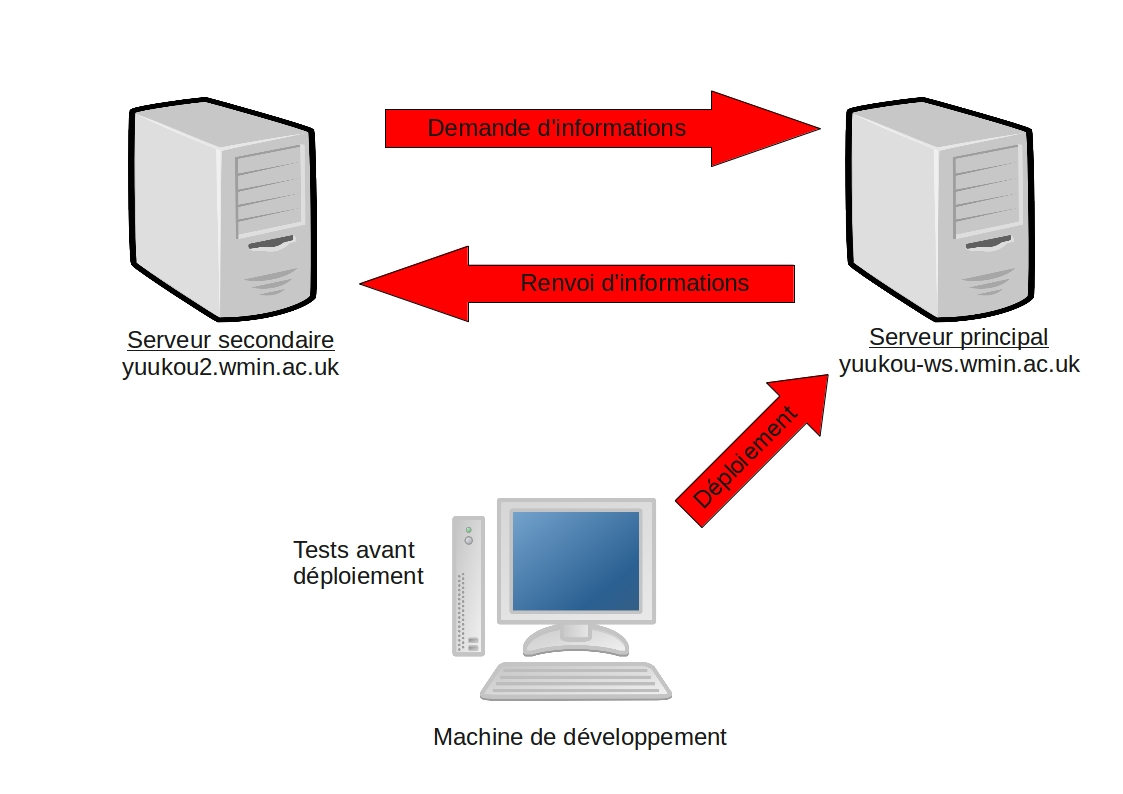
\includegraphics[scale=0.35]{gestionProjet.jpg}
	\caption{Sch\'ema de la gestion du projet}
	\label{figure:gestionProjet}

\end{figure}

Le serveur principal poss\`ede un syst\`eme d'exploitation Debian version 6.0.5 (\textit{Squeeze}) et h\'eberge le service Web dans une version stable ainsi que tous les outils n\'ecessaire \`a son fonctionnement comme le serveur de gestion de base de donn\'ees (SGBD) MySQL, une version de Java \`a jour, le serveur d'application GlassFish mais aussi Nagios.
La faible consommation CPU de Nagios dans la surveillance des machines de l'universit\'e fait, qu'actuellement, il peut \^etre h\'eberg\'e sur le m\^eme serveur que le service Web.
Le serveur principal h\'eberge aussi le gestionnaire de version subversion (SVN) sur lequel est constamment maintenu le projet.
Il est accessible sur le r\'eseau sous le nom de domaine \textsf{yuukou-ws.wmin.ac.uk}.

Le serveur dit {\og}secondaire{\fg} poss\`ede lui aussi le m\^eme syst\`eme d'exploitation Debian et h\'eberge l'application Web permettant de communiquer avec le service Web.
Cette application fait r\'eguli\`erement appel au service Web pour obtenir les informations dont elle a besoin pour afficher correctement ses pages.
Il est accessible sur le r\'eseau sous le nom de domaine \textsf{yuukou2.wmin.ac.uk}.

La machine de d\'eveloppement poss\`ede un syst\`eme d'exploitation Linux Mint version 11 (\textit{Katya}), tous les outils n\'ecessaires au d\'eveloppement (comme Java, NetBeans, \ldots), mais aussi un serveur de gestion de base de donn\'ee (SGBD) MySQL et un serveur GlassFish, tous deux servant \`a effectuer des tests avant d\'eploiement.
\`A chaque d\'eploiement sur le serveur principal, la version du projet est publi\'ee sur le SVN afin de garantir une s\'ecurit\'e dans le cas d'une r\'egression dans le d\'eveloppement.


\section{Gestion de la base de donn\'ees}

\subsection{Structure de la base de donn\'ees}



\subsection{Explications}

\subsection{G\'en\'eration de la configuration Nagios \`a partir de la base de donn\'ees}

\section{Le service Web}

\subsection{Mise en place}

\subsection{Le cycle principal}
\label{section:cyclePrincipal}

\subsection{Les fonctionnalit\'es publiques}

\subsection{Les fonctionnalit\'es priv\'ees}

\subsection{Le retour des informations}

\subsection{S\'ecurisation du service Web}
\label{section:securisation}

\subsubsection{Explications}

La s\'ecurit\'e est un point important dans l'acc\`es \`a un service Web. 
Les donn\'ees transmises par \YuukouII{} contiennent des informations sur la structure des diff\'erents campus mais aussi des informations sur les \'etudiants (nom, pr\'enom, photo par exemple).
Il est donc important de limiter l'acc\'es aux donn\'ees mais aussi de s\'ecuriser toutes les communications.
C'est dans cet optique, qu'il a \'et\'e d\'ecid\'e de mettre en place le protocole SSL entre le service Web et toute application voulant communiquer avec.

Le protocol Secure Sockets Layer, ou SSL, est con\c{c}u pour assurer la confidentialit\'e des \'echanges entre un client et un serveur Web, sur diff\'erents protocoles de transport (en g\'en\'eral HTTP).
Les sites Internet b\'en\'eficiant de ce protocole sont reconnaissables du fait de leurs URL\protect\footnote{\textit{Uniform Resource Locator}} commen\c{c}ant par \textsf{https://} o\`u le 's' signifie \textit{secured}.



\subsubsection{Mise en place}

La mise en place d'un protocole SSL sur une service Web via NetBeans et GlassFish est tr\`es facile \`a mettre en place.
Il suffit pour cela de configurer

\subsubsection{Fonctionnement}


\section{Catalogue logiciels des salles}

\section{Gestion de l'emploi du temps}

\subsection{Les flux RSS de l'universit\'e}

\subsection{Correspondance des salles}

\section{Tests du service Web}

\subsection{Mise en place d'un client}

\subsection{Consommation les m\'ethodes}

\section{Am\'eliorations possibles}

\section{Travail en \'equipe}

\section{Probl\`emes rencontr\'es}

\section{Calendrier du stage}
Arriv\'ee : Lundi 13 F\'evrier
D\'epart : Lundi 4 Juin

semaine 1 : Arriv\'ee et d\'ecouverte du projet, premier entretien avec l'\'equipe technique et leurs attentes
semaine 2 : D\'ecouverte des services Web 
semaine 3 : Conception de la base de donn\'ees et d\'ebut d'impl\'ementation du cycle principal de l'application
semaine 4 : fin d'impl\'ementation du cycle principal
semaine 5 : Mise en place de l'emploi du temps + mise en place de SSL
semaine 6 : D\'eveloppement des premi\`eres m\'ethodes Web + fin de mise en place de SSL
semaine 7 : Mise en place du syst\`eme JSON
semaine 8 : 
semaine 9 : 
semaine 10 : D\'ebut de r\'edaction du rapport
semaine 11 : 
semaine 12 : 
semaine 13 : R\'ecup\'eration du catalogue de logiciels de M\'ediaWiki
semaine 14 : Ajout de m\'ethodes Web et am\'elioration du chargement de la base de donn\'ees
semaine 15 : r\'edaction du rapport de stage et maintenance des fonctionnalit\'es du service Web
semaine 16 : fin d'\'ecriture du rapport de stage

\section{R\'ecapitulatif du projet}

La figure~\ref{figure:yuukouEtYuukouII} permet de donner une vue d'ensemble sur les principales fonctionnalit\'es dont le projet dispose.
Les cadres pleins repr\'esentent des fonctionnalit\'es dont le principe a \'et\'e repris de {\Yuukou}, les cadres en pointill\'es quant \`a eux, repr\'esentent les nouvelles fonctionnalit\'es qu'apporte \YuukouII.

\begin{figure}[!ht]
	\centering
	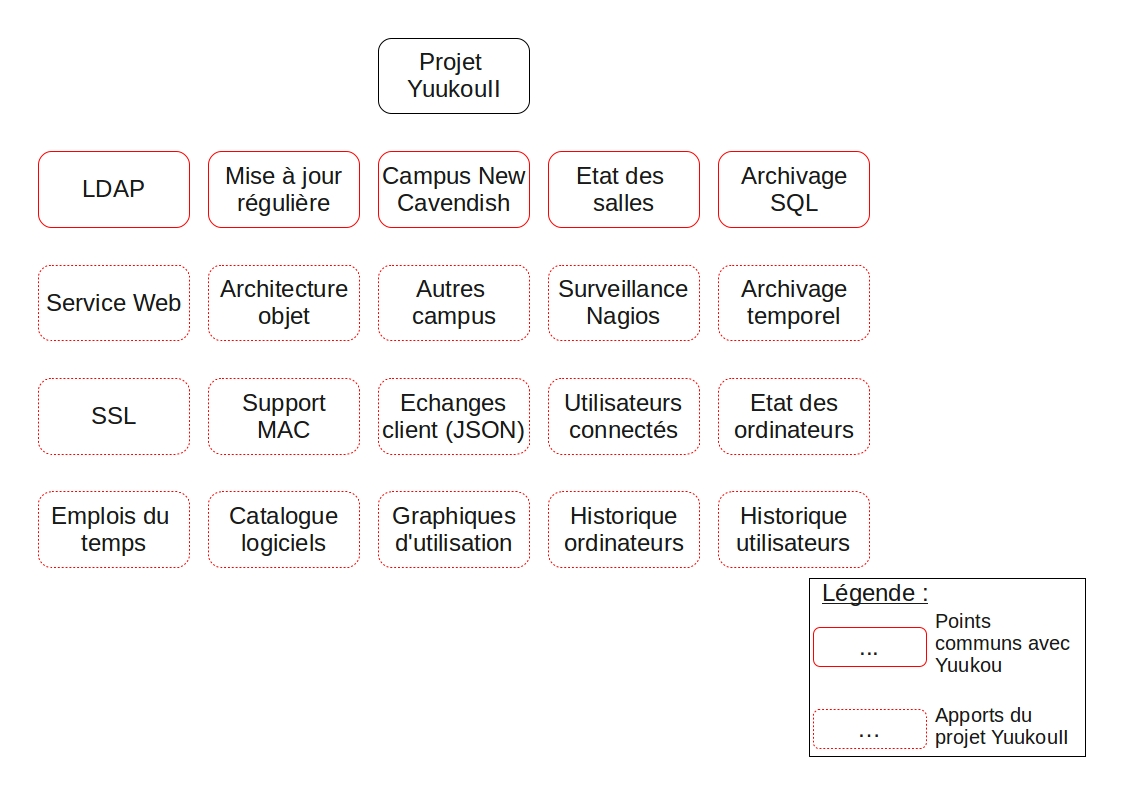
\includegraphics[scale=0.375]{yuukouEtYuukouII.jpg}
	\caption{R\'ecapitulatif des fonctionnalit\'es reprises de {\Yuukou} et les nouvelles de \YuukouII}
	\label{figure:yuukouEtYuukouII}

\end{figure}



\clearpage
